\section{问题一：自由轮廓布局模型的建立与求解}

本问以可旋转二维矩形装箱描述硬模块布局，并以外接面积和轮廓长短边比构成词典序目标~\cite{wong1989}。求解时将未知自由轮廓转化为候选宽度搜索，由 Skyline 与 MaxRects 构造候选布局，再按目标顺序筛选。

\subsection{几何模型：可旋转二维矩形装箱}

\subsubsection{模块位置与旋转状态}

设硬模块集合为 $\mathcal{B}=\{1,2,\ldots,n\}$，模块 $i$ 的原始尺寸为 $(w_i^0,h_i^0)$，旋转状态为 $r_i$，左下角坐标为 $(x_i,y_i)$。旋转后的尺寸为
\begin{equation}
  (w_i,h_i)=
  \begin{cases}
    (w_i^0,h_i^0), & r_i=0,\\
    (h_i^0,w_i^0), & r_i=1.
  \end{cases}
  \label{eq:q1_rotation}
\end{equation}
其中 $r_i\in\{0,1\}$，且 $x_i,y_i\ge0$。

\subsubsection{模块非重叠与外接轮廓}

对任意两个不同模块 $i,j\in\mathcal{B}$，它们必须分别位于对方的左、右、下、上四种相对位置之一，即
\begin{equation}
  x_i+w_i\le x_j
  \ \vee\ 
  x_j+w_j\le x_i
  \ \vee\ 
  y_i+h_i\le y_j
  \ \vee\ 
  y_j+h_j\le y_i,
  \qquad i<j.
  \label{eq:q1_nonoverlap}
\end{equation}
外接轮廓左下角归一化为原点，其宽、高及面积为
\begin{equation}
  W=\max_{i\in\mathcal{B}}(x_i+w_i),\qquad
  H=\max_{i\in\mathcal{B}}(y_i+h_i),\qquad
  A_{\mathrm{box}}=WH.
  \label{eq:q1_outline}
\end{equation}
模块总面积为
\begin{equation}
  A_{\mathrm{block}}=\sum_{i\in\mathcal{B}}w_i^0h_i^0
  \label{eq:q1_area_lb}
\end{equation}
并满足 $A_{\mathrm{box}}\ge A_{\mathrm{block}}$。

\subsubsection{布局评价与优化目标}

定义长短边比和面积冗余率为
\begin{equation}
  \rho=\frac{\max(W,H)}{\min(W,H)},\qquad
  \eta=\frac{A_{\mathrm{box}}-A_{\mathrm{block}}}{A_{\mathrm{block}}}.
  \label{eq:q1_metrics}
\end{equation}

相应的词典序目标为
\begin{equation}
  \operatorname*{lex\,min}_{\{x_i,y_i,r_i\}}
  \left(A_{\mathrm{box}},\rho\right),
  \quad \text{s.t. 式~\eqref{eq:q1_rotation}--\eqref{eq:q1_nonoverlap}}.
  \label{eq:q1_lex_objective}
\end{equation}
程序内部使用下式比较候选方案：
\begin{equation}
  F=A_{\mathrm{box}}+\frac{|W-H|}{\max(W,H)}.
  \label{eq:q1_scalar_score}
\end{equation}
由于整数布局的 $A_{\mathrm{box}}$ 为整数，而第二项位于 $[0,1)$ 且随 $\rho$ 单调增加，$F$ 仅是实现词典序比较的内部评价量，\textbf{不替代}式~\eqref{eq:q1_lex_objective}所定义的原始优化目标。

\subsection{求解方法：轮廓宽度搜索与启发式装箱}

由旋转对称性可令候选轮廓满足 $W\le H$。整数宽度搜索从
\begin{equation}
  W_{\min}=\max_{i\in\mathcal{B}}\min(w_i^0,h_i^0),
  \label{eq:q1_width_lb}
\end{equation}
开始；若当前最小外接面积为 $A_{\mathrm{best}}$，仍可能改进面积的候选短边满足
\begin{equation}
  W\le \sqrt{A_{\mathrm{box}}}<\sqrt{A_{\mathrm{best}}}.
  \label{eq:q1_width_ub}
\end{equation}
故从 $W_{\min}$ 起逐一考察整数宽度，并随更小的 $A_{\mathrm{best}}$ 动态收紧上界。对每个候选宽度，按少量面积或边长顺序组织模块，分别用 Skyline~\cite{wei2011} 维护上边界、用 MaxRects~\cite{jylanki2010} 利用剩余矩形空间；\texttt{n300} 因规模较大仅采用 Skyline 全宽度扫描。所有候选最终统一由式~\eqref{eq:q1_lex_objective}的顺序筛选，形成“轮廓宽度搜索—启发式布局构造—方案筛选”的求解主线。

\subsection{求解结果与分析}
表~\ref{tab:q1_results}汇总三组实例的外接轮廓及其面积、形状指标。

\begin{table}[H]
  \centering
  \caption{问题一三组芯片的布局结果}
  \label{tab:q1_results}
  \small
  \resizebox{\textwidth}{!}{%
  \begin{tabular}{lrrrrrrr}
    \toprule
    实例 & 模块数 & $A_{\mathrm{block}}$ & $W$ & $H$ & $A_{\mathrm{box}}$ & $\eta/\%$ & $\rho$ \\
    \midrule
    \texttt{n100} & 100 & 179501 & 86  & 2155 & 185330 & 3.2473 & 25.0581 \\
    \texttt{n200} & 200 & 175696 & 60  & 3015 & 180900 & 2.9619 & 50.2500 \\
    \texttt{n300} & 300 & 273170 & 520 & 557  & 289640 & 6.0292 & 1.0712 \\
    \bottomrule
  \end{tabular}%
  }
\end{table}

三组结果并非沿两个指标同步改善。\texttt{n100} 与 \texttt{n200} 的面积冗余率均约为 $3\%$，说明模块总面积之外仅增加了较少空隙；但其长短边比分别达到 $25.0581$ 和 $50.2500$，紧凑面积对应的是显著拉长的轮廓。为兼顾真实形状与局部可读性，图~\ref{fig:q1_n100_n200}左侧保留真实比例总览，右侧按纵坐标连续分段展开，所有分段均直接来自同一组冻结坐标。

\begin{figure}[H]
  \centering
  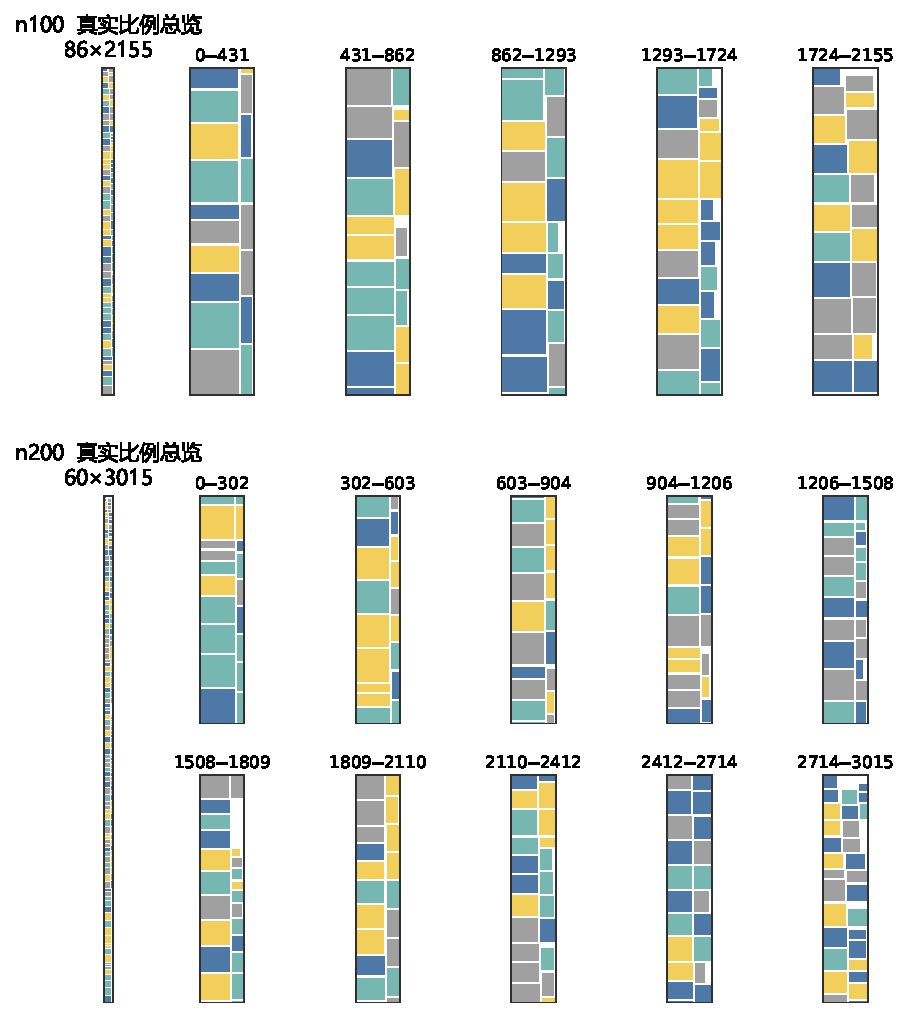
\includegraphics[width=\textwidth]{../results/q1/figures/q1_slender_overview_segments.pdf}
  \caption{\texttt{n100} 与 \texttt{n200} 的真实比例总览及分段展开。左列呈现完整外接轮廓，右侧依次展示连续纵向区段；低饱和颜色仅用于区分相邻模块。}
  \label{fig:q1_n100_n200}
\end{figure}

相对而言，\texttt{n300} 的 $520\times557$ 轮廓接近正方形，长短边比仅为 $1.0712$；与此同时，其面积冗余率上升至 $6.0292\%$。其真实比例布局见图~\ref{fig:q1_n300}。

\begin{figure}[H]
  \centering
  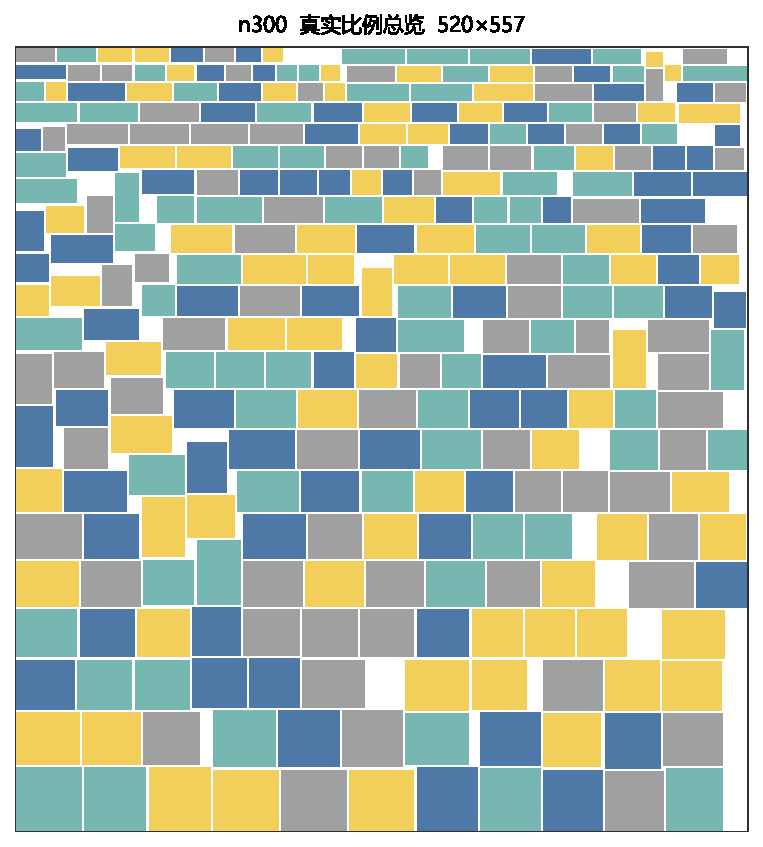
\includegraphics[width=0.78\textwidth]{../results/q1/figures/q1_n300_balanced_layout.pdf}
  \caption{\texttt{n300} 的真实比例布局。$520\times557$ 外接轮廓接近正方形，白色区域为模块间空隙。}
  \label{fig:q1_n300}
\end{figure}

综合三组实例，较低的面积冗余率并未保证接近正方形的外形，而更均衡的轮廓也可能伴随更高的面积冗余。由此可见，在本组自由轮廓算例中，\textbf{面积紧凑性与轮廓均衡性存在竞争关系}；词典序目标所规定的主次顺序，正是三组布局呈现不同形态的直接判优依据。

\subsection{模型结果检验}

最终坐标均通过模块完整性、两两非重叠和模块总面积一致性复核。Skyline 与 MaxRects 属于启发式构造，因此表~\ref{tab:q1_results}给出的是当前搜索范围内的可行上界，不能据此严格证明大规模实例的全局最优性。

至此，本问在保持面积优先判据的同时揭示了紧凑性与均衡性的竞争规律；所建立的模块旋转、非重叠约束与轮廓表示，也为后续加入固定边界、互连关系或形状扩展提供了基础。
